\documentclass{article}\usepackage[]{graphicx}\usepackage[]{xcolor}
% maxwidth is the original width if it is less than linewidth
% otherwise use linewidth (to make sure the graphics do not exceed the margin)
\makeatletter
\def\maxwidth{ %
  \ifdim\Gin@nat@width>\linewidth
    \linewidth
  \else
    \Gin@nat@width
  \fi
}
\makeatother

\definecolor{fgcolor}{rgb}{0.345, 0.345, 0.345}
\newcommand{\hlnum}[1]{\textcolor[rgb]{0.686,0.059,0.569}{#1}}%
\newcommand{\hlsng}[1]{\textcolor[rgb]{0.192,0.494,0.8}{#1}}%
\newcommand{\hlcom}[1]{\textcolor[rgb]{0.678,0.584,0.686}{\textit{#1}}}%
\newcommand{\hlopt}[1]{\textcolor[rgb]{0,0,0}{#1}}%
\newcommand{\hldef}[1]{\textcolor[rgb]{0.345,0.345,0.345}{#1}}%
\newcommand{\hlkwa}[1]{\textcolor[rgb]{0.161,0.373,0.58}{\textbf{#1}}}%
\newcommand{\hlkwb}[1]{\textcolor[rgb]{0.69,0.353,0.396}{#1}}%
\newcommand{\hlkwc}[1]{\textcolor[rgb]{0.333,0.667,0.333}{#1}}%
\newcommand{\hlkwd}[1]{\textcolor[rgb]{0.737,0.353,0.396}{\textbf{#1}}}%
\let\hlipl\hlkwb

\usepackage{framed}
\makeatletter
\newenvironment{kframe}{%
 \def\at@end@of@kframe{}%
 \ifinner\ifhmode%
  \def\at@end@of@kframe{\end{minipage}}%
  \begin{minipage}{\columnwidth}%
 \fi\fi%
 \def\FrameCommand##1{\hskip\@totalleftmargin \hskip-\fboxsep
 \colorbox{shadecolor}{##1}\hskip-\fboxsep
     % There is no \\@totalrightmargin, so:
     \hskip-\linewidth \hskip-\@totalleftmargin \hskip\columnwidth}%
 \MakeFramed {\advance\hsize-\width
   \@totalleftmargin\z@ \linewidth\hsize
   \@setminipage}}%
 {\par\unskip\endMakeFramed%
 \at@end@of@kframe}
\makeatother

\definecolor{shadecolor}{rgb}{.97, .97, .97}
\definecolor{messagecolor}{rgb}{0, 0, 0}
\definecolor{warningcolor}{rgb}{1, 0, 1}
\definecolor{errorcolor}{rgb}{1, 0, 0}
\newenvironment{knitrout}{}{} % an empty environment to be redefined in TeX

\usepackage{alltt}
\usepackage{amsmath} %This allows me to use the align functionality.
                     %If you find yourself trying to replicate
                     %something you found online, ensure you're
                     %loading the necessary packages!
\usepackage{amsfonts}%Math font
\usepackage{graphicx}%For including graphics
\usepackage{hyperref}%For Hyperlinks
\usepackage[shortlabels]{enumitem}% For enumerated lists with labels specified
                                  % We had to run tlmgr_install("enumitem") in R
\hypersetup{colorlinks = true,citecolor=black} %set citations to have black (not green) color
\usepackage{natbib}        %For the bibliography
\setlength{\bibsep}{0pt plus 0.3ex}
\bibliographystyle{apalike}%For the bibliography
\usepackage[margin=0.50in]{geometry}
\usepackage{float}
\usepackage{multicol}

%fix for figures
\usepackage{caption}
\newenvironment{Figure}
  {\par\medskip\noindent\minipage{\linewidth}}
  {\endminipage\par\medskip}
\IfFileExists{upquote.sty}{\usepackage{upquote}}{}
\begin{document}

\vspace{-1in}
\title{Lab 1 -- MATH 240 -- Computational Statistics}

\author{
  Anya Suko \\
  Computational Statistics  \\
  Math  \\
  {\tt asuko@colgate.edu}
}

\date{}

\maketitle

\begin{multicols}{2}
\begin{abstract}
This document provides a basic template for the 2-page labs we will complete each week. Here, you should provide a succint sumary about what you did and why it might be helpful. 
\end{abstract}

\noindent \textbf{Keywords:} What topics does the lab cover with respect to class? 

\section{Instructions}
For this lab, you will
\begin{enumerate}[1.]\itemsep0em
  \item Install \href{https://cran.r-project.org/bin/windows/base/}{R}. and \href{https://posit.co/download/rstudio-desktop/}{RStudio}.
  \item Install tinytex (if necessary): \\ \texttt{install.packages("tinytex")}
  \item Create a GitHub account \href{https://github.com/}{here}, and email me your user-name
  \item Install \href{https://desktop.github.com/}{GitHub desktop}
  \item Accept the LAB 1 assignment \href{https://classroom.github.com/a/gfC_xMMl}{here}.
  \item recreate this document (except put your name/info at the top) to get used to writing in LATEX and to see the types of things we can do when creating a document to convey statistical information. make sure to commit and push your work to GitHub desktop as you finish each section.
\end{enumerate}

\noindent\textbf{Remark}
\noindent You will find the class Sweave cheatsheet to be \emph{incredibly} helpful.

\section{Word Processing Tasks}

\subsection{Centering Text}
\begin{center}
We can center text in Sweave.
\end{center} 

\subsection{Bold, Italics, and Underlining}
We can \textbf{bold}, \textit{italicize}, \underline{underline}, and \emph{emphasize} text in Sweave.

Note, I did a column break here so that the list wasn't broken across columns.\columnbreak 

\subsection{Lists, and Numbered Lists}
We can write an unordered list in Sweave
\begin{itemize}\itemsep0em
\item first item
\item second item
\item third item
\end{itemize}
We can write a numbered list in Sweave
\begin{enumerate}[1.]\itemsep0em
\item first item
\item second item
\item third item
\end{enumerate}
We can write a lettered list in Sweave
\begin{enumerate}[a.]\itemsep0em
\item first item
\item second item
\item third item
\end{enumerate}

\subsection{Submissions}
This part of the midterm is due Sunday November 14 by 5p. I will not accept late submissions. Note that you may use this template to help build your introduction and methods sections, and you can use the work you did as a group during the datathon. Still, I expect this submission to be your own summary and extension of that work without collaboration.

\subsection{Typing Mathematial Equations}
We can write a one line equation that is centered like this
\[\widehat{y_i} = \beta_0 + \beta_1 x_{1i}+ \beta_2 x_{2i} +  \beta_3 x_{1i} x_{2i} + \epsilon_i.\]
This can be written in the text, as $\widehat{y_i} = \beta_0 + \beta_1 x_{1i}+ \beta_2 x_{2i} +  \beta_3 x_{1i} x_{2i} + \epsilon_i$. using as well.

To create a multi-line equation that is centered like this
\begin{align*}
8(x-5)+x &=9(x-5)+5 \\
8x-40+x &=9x-45+5 \tag{Distributing}\\
9x-40 &= 9x-40 \tag{combining like terms}\\
9x &=9x \tag{adding 40 to both sides}\\
x &=x \tag{dividing both sides by 9}
\end{align*}
The equality holds for any z.

Note, I did a page break here so that the next section started on a clean page. \pagebreak
\subsection{Running R Code}
Code chunks can be entered into Sweave; e.g, here are some comments.
\begin{knitrout}\scriptsize
\definecolor{shadecolor}{rgb}{0.969, 0.969, 0.969}\color{fgcolor}\begin{kframe}
\begin{alltt}
\hlcom{# R code goes here}
\hlcom{# Output is automatically printed in the pdf}
\end{alltt}
\end{kframe}
\end{knitrout}

Below, you can see that we can do algebra with R.
\begin{knitrout}\scriptsize
\definecolor{shadecolor}{rgb}{0.969, 0.969, 0.969}\color{fgcolor}\begin{kframe}
\begin{alltt}
\hlnum{8}\hlopt{*}\hldef{(}\hlnum{9}\hlopt{-}\hlnum{5}\hldef{)}\hlopt{+}\hlnum{9} \hlcom{#8(x-5)+x for x=9}
\end{alltt}
\begin{verbatim}
## [1] 41
\end{verbatim}
\end{kframe}
\end{knitrout}

Below, we show we can produce the code without evaluating it.
\begin{knitrout}\scriptsize
\definecolor{shadecolor}{rgb}{0.969, 0.969, 0.969}\color{fgcolor}\begin{kframe}
\begin{alltt}
\hlnum{8}\hlopt{*}\hldef{(}\hlnum{9}\hlopt{-}\hlnum{5}\hldef{)}\hlopt{+}\hlnum{9} \hlcom{#8(x-5)+x for x=9}
\hlcom{## [1] 41}
\end{alltt}
\end{kframe}
\end{knitrout}

Alternatively, we can produce the output without the code.
\begin{knitrout}\scriptsize
\definecolor{shadecolor}{rgb}{0.969, 0.969, 0.969}\color{fgcolor}\begin{kframe}
\begin{verbatim}
## [1] 41
\end{verbatim}
\end{kframe}
\end{knitrout}

We can also call object values from R directly.
\begin{knitrout}\scriptsize
\definecolor{shadecolor}{rgb}{0.969, 0.969, 0.969}\color{fgcolor}\begin{kframe}
\begin{alltt}
\hldef{result} \hlkwb{<-} \hlnum{8}\hlopt{*}\hldef{(}\hlnum{9}\hlopt{-}\hlnum{5}\hldef{)}\hlopt{+}\hlnum{0} \hlcom{#8(x-5)+x for x=9}
\hldef{result.with.error} \hlkwb{<-} \hldef{result} \hlopt{+} \hlkwd{rnorm}\hldef{(}\hlnum{1}\hldef{,}\hlkwc{mean}\hldef{=}\hlnum{0}\hldef{,}\hlkwc{sd}\hldef{=}\hlnum{0.1}\hldef{)}
\hldef{result.with.error}
\end{alltt}
\begin{verbatim}
## [1] 32.02352
\end{verbatim}
\end{kframe}
\end{knitrout}
\subsection{Plotting}
We can also plot with R.
\begin{knitrout}\scriptsize
\definecolor{shadecolor}{rgb}{0.969, 0.969, 0.969}\color{fgcolor}\begin{kframe}
\begin{alltt}
\hlcom{#Plot a histogram of random exponential data}
\hlkwd{hist}\hldef{(}\hlkwd{rexp}\hldef{(}\hlnum{100}\hldef{))}
\end{alltt}
\end{kframe}
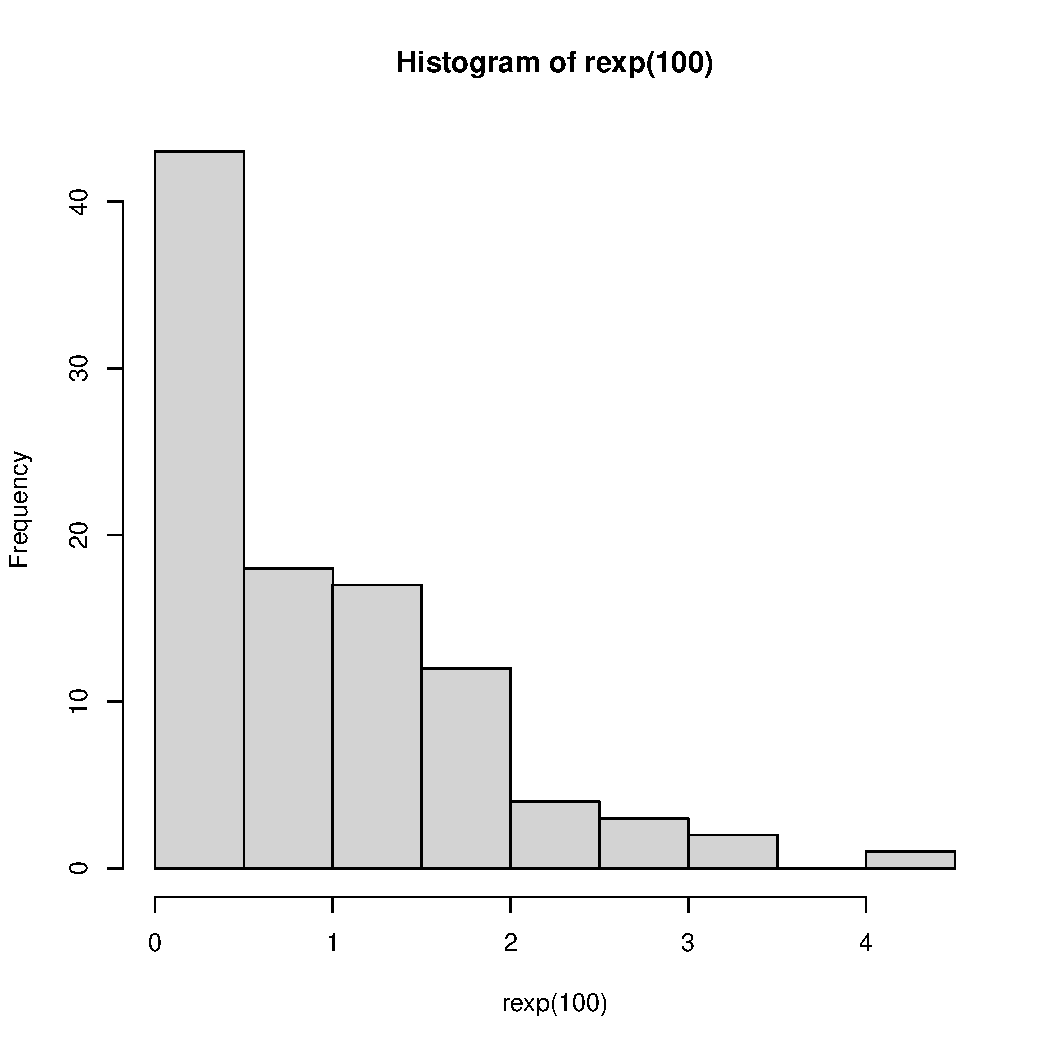
\includegraphics[width=\maxwidth]{figure/unnamed-chunk-6-1} 
\end{knitrout}
Figure 1: A histogram of random exponentially distributed data, n=100
\subsection{Tables}
Below, we load and take a peek at some data about the death rates per 1000 in Virginia in 1940 (Molyneaux et al., 1947).
\begin{knitrout}\scriptsize
\definecolor{shadecolor}{rgb}{0.969, 0.969, 0.969}\color{fgcolor}\begin{kframe}
\begin{alltt}
\hlkwd{data}\hldef{(}\hlsng{"VADeaths"}\hldef{)}
\hlkwd{head}\hldef{(VADeaths)} \hlcom{#take a peek of the data}
\end{alltt}
\begin{verbatim}
##       Rural Male Rural Female Urban Male Urban Female
## 50-54       11.7          8.7       15.4          8.4
## 55-59       18.1         11.7       24.3         13.6
## 60-64       26.9         20.3       37.0         19.3
## 65-69       41.0         30.9       54.6         35.1
## 70-74       66.0         54.3       71.1         50.0
\end{verbatim}
\end{kframe}
\end{knitrout}
\indent If we want to print this nicely, we can do so using the xtable packagr (Dahl et al., 2019), which we can refrence using the label (Table 1).
\begin{kframe}
\begin{alltt}
\hlkwd{library}\hldef{(xtable)}
\hlkwd{colnames}\hldef{(VADeaths)}\hlkwb{<-}\hlkwd{c}\hldef{(}\hlsng{"Rural Male"}\hldef{,}\hlsng{"Rural Female"}\hldef{,}\hlsng{"Urban Male"}\hldef{,}\hlsng{"Rural Female"}\hldef{)}
\hldef{VADeaths.table}\hlkwb{<-}\hlkwd{xtable}\hldef{(VADeaths,}\hlkwc{label} \hldef{=} \hlsng{"VADeaths.tab"}\hldef{)}
\hlkwd{print}\hldef{(VADeaths.table,}
\hlkwc{table.placement} \hldef{=} \hlsng{"H"}\hldef{,} \hlkwc{include.rownames}\hldef{=}\hlnum{FALSE}\hldef{,} \hlkwc{size} \hldef{=} \hlsng{"small"}\hldef{)}
\end{alltt}
\end{kframe}% latex table generated in R 4.4.2 by xtable 1.8-4 package
% Tue Jan 28 14:11:20 2025
\begin{table}[H]
\centering
\begingroup\small
\begin{tabular}{rrrr}
  \hline
Rural Male & Rural Female & Urban Male & Rural Female \\ 
  \hline
11.70 & 8.70 & 15.40 & 8.40 \\ 
  18.10 & 11.70 & 24.30 & 13.60 \\ 
  26.90 & 20.30 & 37.00 & 19.30 \\ 
  41.00 & 30.90 & 54.60 & 35.10 \\ 
  66.00 & 54.30 & 71.10 & 50.00 \\ 
   \hline
\end{tabular}
\endgroup
\label{VADeaths.tab}
\end{table}

\indent Table 1: Death Rates per 1000 in Virginia
%%%%%%%%%%%%%%%%%%%%%%%%%%%%%%%%%%%%%%%%%%%%%%%%%%%%%%%%%%%%%%%%%%%%%%%%%%%%%%%%
% Bibliography
%%%%%%%%%%%%%%%%%%%%%%%%%%%%%%%%%%%%%%%%%%%%%%%%%%%%%%%%%%%%%%%%%%%%%%%%%%%%%%%%
\vspace{2em}

\noindent\textbf{Bibliography:} Note that when you add citations to your bib.bib file \emph{and}
you cite them in your document, the bibliography section will automatically populate here.

\begin{tiny}
\bibliography{bib}
\end{tiny}
\end{multicols}

%%%%%%%%%%%%%%%%%%%%%%%%%%%%%%%%%%%%%%%%%%%%%%%%%%%%%%%%%%%%%%%%%%%%%%%%%%%%%%%%
% Appendix
%%%%%%%%%%%%%%%%%%%%%%%%%%%%%%%%%%%%%%%%%%%%%%%%%%%%%%%%%%%%%%%%%%%%%%%%%%%%%%%%
\newpage
\onecolumn
\section{Appendix}

If you have anything extra, you can add it here in the appendix. This can include images or tables that don't work well in the two-page setup, code snippets you might want to share, etc.

\end{document}
